\appendix
\section{Anhang}
\subsection{Anforderungen der DB AG}
Anforderungen an die Transformatoren aus der Technischen Spezifikation der Frequenzumrichter
der DB AG vom 07.05.2009: 
"5.9 Transformatoren und Trafowannen“

\subsubsection*{Korrosionsschutz (Anstrich)}
Zur Gewährleistung der Mindestlebenserwartung von 30 Jahren ist eine Oberflächenbehandlung von Kessel, Ausdehnungsgefäß, Radiatoren und Rohrleitungen notwendig. Die Anstriche sind nach TL 918 300, Bl. 87 auszuführen. Korrosionsbeständige Bauteile sind ebenfalls in die Oberflächenbehandlung mit einzubeziehen (Grund- / Haftbeschichtung und die beiden Deckanstriche).
Feuerverzinkte Bauteile sind besonders sorgfältig zu behandeln.
Die Verwendung von alternativen Farbherstellern oder das Aufbringen von Wasserlacken ist mit der 
DB Energie abzustimmen.

\subsubsection*{Oberflächenbehandlung von Kessel, Ausdehnungsgefäß, Radiatoren und Rohrleitungen}
Die Komponenten sind mit einer Spritzverzinkung in der Mindestschichtendicke von \SI{100}{\um}, nach DIN-VDE 55 928 Teil 5 oder mit einer Epoxyd-Zinkstaubfarbe, DB Mat.-Nr. 687.03, mit einer abschließenden Mindesttrockenschichtdicke von \SI[]{80}{\um}, zu behandeln. Nach dem metallischen Überzug ist eine Grund- / Haftbeschichtung aufzutragen.

\subsubsection*{Erste Deckbeschichtung}
Die erste Deckbeschichtung ist mit Epoxyd-Eisenglimmer Anstrich in der Farbe grau, Farbton DB 702, Mat.-Nr. 687.12, auszuführen. Die Mindesttrockenschichtdicke beträgt \SI{80}{\um}.

\subsubsection*{Zweite Deckbeschichtung}
Die zweite Deckbeschichtung ist mit PUR-Eisenglimmer Anstrich in der Farbe grün, Farbton DB 601, Mat.-Nr. 687.61, auszuführen. Die Mindesttrockenschichtdicke beträgt \SI{80}{\um}.

\subsubsection*{Dichtigkeit}
Für die Öldichtigkeit beträgt die Verjährungsfrist für Sachmängel 5 Jahre nach Inbetriebnahme.
Desgleichen beträgt die Verjährungsfrist für Sachmängel 5 Jahre für den aufgebrachten Korrosionsschutz

\subsubsection*{Beschilderung}
Die Beschilderung der Armaturen hat entsprechend DIN 42513 “Bauteilkennzeichnung für Transformatoren und Drosselspulen“ zu erfolgen. Es sind alterungsbeständige Kennzeichnungsschilder zu verwenden.

\subsubsection*{Alterungsbeständigkeit}
Alle eingesetzten Kunststoffe müssen UV-, alterungs- und wetterbeständig ausgeführt sein. Dies gilt insbesondere für eingesetzte Kabel, Kabelbinder und angebrachte Kennzeichnungsschilder.

\subsubsection*{Überspannungsschutz}
Für den Überspannungsschutz der Umrichtertrafos und -komponenten sind auf der 50-Hz- und 16,7-Hz-Seite Metalloxid-Überspannungsableiter vorzusehen. Sollten diese aus Sicht des Herstellers nicht notwendig sein, ist dies schriftlich gegenüber dem Auftraggeber zu begründen (Siehe auch 7.3).

\subsubsection*{Absturzsicherung}
Für alle Bauteile (Trafos, Container, etc.) ist eine Absturzsicherung mitzuliefern. Die Bestimmungen des Arbeitsschutzes sind einzuhalten.

\subsubsection*{Luftabschluss}
Alle Transformatoren sind mit Luftabschlusssystemen (Luftsack, Ausdehnung über Radiatoren) zu versehen.

\subsubsection*{Transformator - Ölauffangwanne}
Ausführung gemäß den gelten Gesetzen (z. B. Wasserhaushaltsgesetz) als Fertigwannen. Transformatorenfundament aus werksmäßig hergestellten Fertigelementen aus Stahlbeton gem. DIN 1045 C35/45 FD mit den Expositionsklassen XC4, XF3, XA2, Dichtigkeitsnachweis gem. DafStb-Richtlinie “Betonbau beim Umgang mit Wassergefährdenden Stoffen“, monolithisch hergestellt, Boden und Umfassungswände fugenlos aus einem Guss. Die Auffangwannen erfüllen die Anforderungen des Wasserhaushaltsgesetzes (WHG) §19."
\subsection{Harmonische von Umrichterspannungen und Umrichterströmen}
\subsubsection{Oberschwingungsamplituden der Drehstromseite}
Unten werden die maximalen Oberschwingungsamplituden bk der Spannung angegeben, die vom Umrichter an den umrichterseitigen Wicklungssystemen des Drehstromtransformators eingeprägt werden. Der zugehörige Zeitverlauf ergibt sich aus:

\begin{equation*}
    u_\mathrm{k}(t)=b_\mathrm{k}sin(k\cdot \Omega t)
\end{equation*}

\begin{figure}[htb]
    \centering
    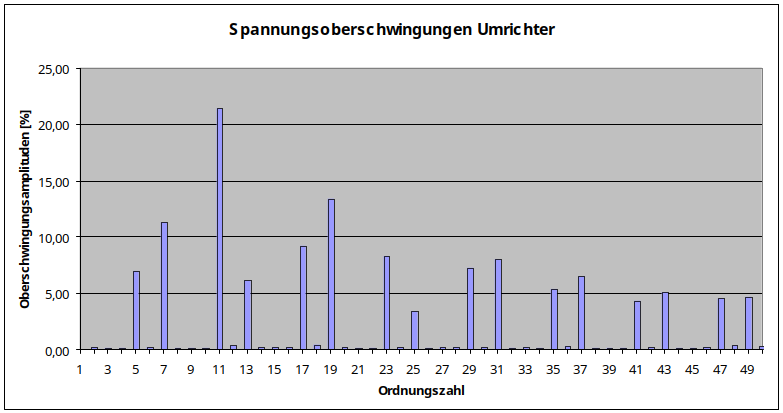
\includegraphics[width=\textwidth]{Bilder/spannungsoberschwingung_umrichter.png}
    \caption{Maximale Oberschwingungsamplituden der Umrichterspannung der Drehstromseite über den Aussteuerungsbereich von 0,9 … 1,1 (100\% entsprechen 3062V verkettet effektiv)}
\end{figure}

\begin{table}[!ht]
    \centering
    \caption[]{Der Gesamt-THD beträgt etwa \SI{29}{\percent} je Wicklung. Die Spannungsamplituden sind zusätzlich als verkettete Effektivwerte angegeben.}
    \begin{tabular}{|l|l|l|}
    \hline
        Ordnungszahl & Oberschwingungsamplitude [\%] & Oberschwingungsamplitude [V] \\ \hline
        5 & 6.98 & 213.72 \\ \hline
        7 & 11.30 & 345.99 \\ \hline
        11 & 21.38 & 654.63 \\ \hline
        13 & 6.15 & 188.30 \\ \hline
        17 & 9.22 & 282.30 \\ \hline
        19 & 13.40 & 410.29 \\ \hline
        23 & 8.28 & 253.52 \\ \hline
        25 & 3.39 & 103.80 \\ \hline
        29 & 7.27 & 222.60 \\ \hline
        31 & 8.01 & 245.26 \\ \hline
        35 & 5.37 & 164.42 \\ \hline
        37 & 6.48 & 198.41 \\ \hline
        41 & 4.33 & 132.58 \\ \hline
        43 & 5.06 & 154.93 \\ \hline
        47 & 4.50 & 137.78 \\ \hline
        49 & 4.64 & 142.07 \\ \hline
        ~ & ~ & ~ \\ \hline
        ~ & ~ & ~ \\ \hline
        Ordnungszahl & Oberschwingungsamplitude [\%] & Oberschwingungsamplitude [V] \\ \hline
        3 & 31.67 & 1119.76 \\ \hline
        9 & 36.02 & 1273.60 \\ \hline
        15 & 15.15 & 535.67 \\ \hline
        21 & 13.43 & 474.85 \\ \hline
        27 & 8.80 & 311.17 \\ \hline
        33 & 9.02 & 318.75 \\ \hline
        39 & 5.40 & 190.97 \\ \hline
        45 & 5.30 & 187.27 \\ \hline
    \end{tabular}
\end{table}
\subsubsection{Oberschwingungsamplituden der Bahnnetzseite}
Die an den umrichterseitigen Wicklungen des Bahnnetztrafos anliegenden Spannungsoberschwingungen sind im nächsten Bild dargestellt. Weiterhin sind die Spannungsoberschwingungen der mittleren Spannung der beiden umrichterseitigen Wicklungen dargestellt. Die Spannungen an den beiden Wicklungen sind zueinander so versetzt, dass sich viele Oberschwingungen in der Summenspannung reduzieren oder auslöschen. Dieser Mittelwert ist die wirksame Gesamtspannung. 

\begin{figure}[htb]
    \centering
    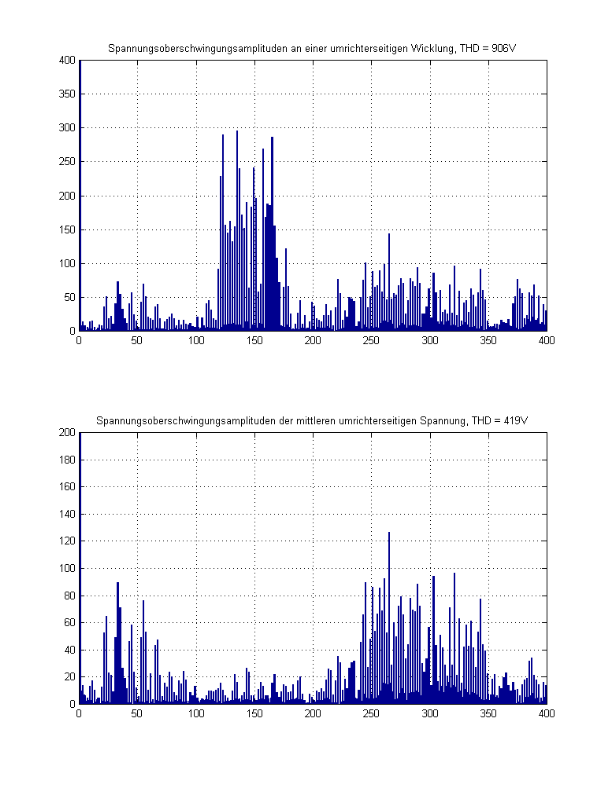
\includegraphics[width=\textwidth]{Bilder/oberschwingungsamp_umrichterseite.png}     
    \caption{Oberschwingungsspektrum der Umrichterspannung der Bahnnetzseite an einer umrichterseitigen Wicklung und mittlere Gesamtspannung der beiden Wicklung}
\end{figure}
\clearpage
\subsection{CAD}
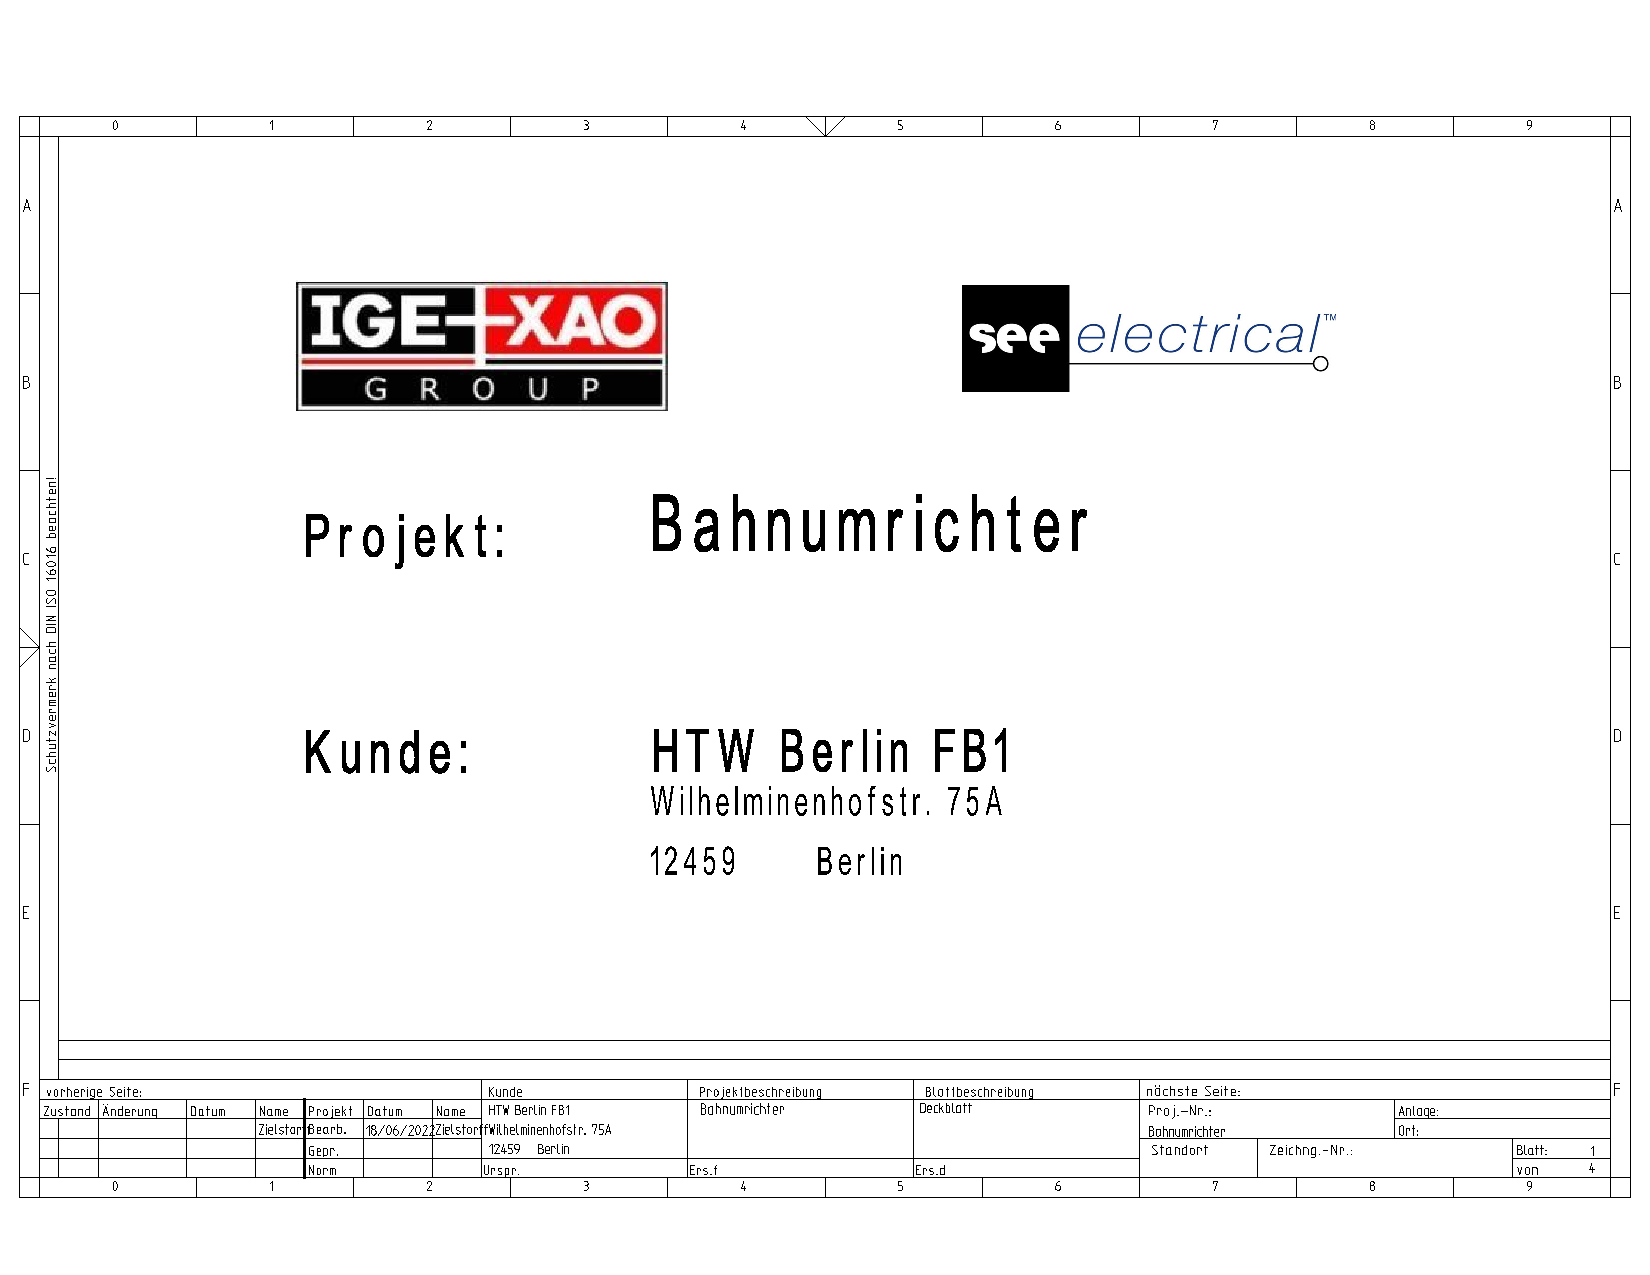
\includepdf[pages=-,landscape]{Bilder/Bahnumrichter_CAD.pdf}
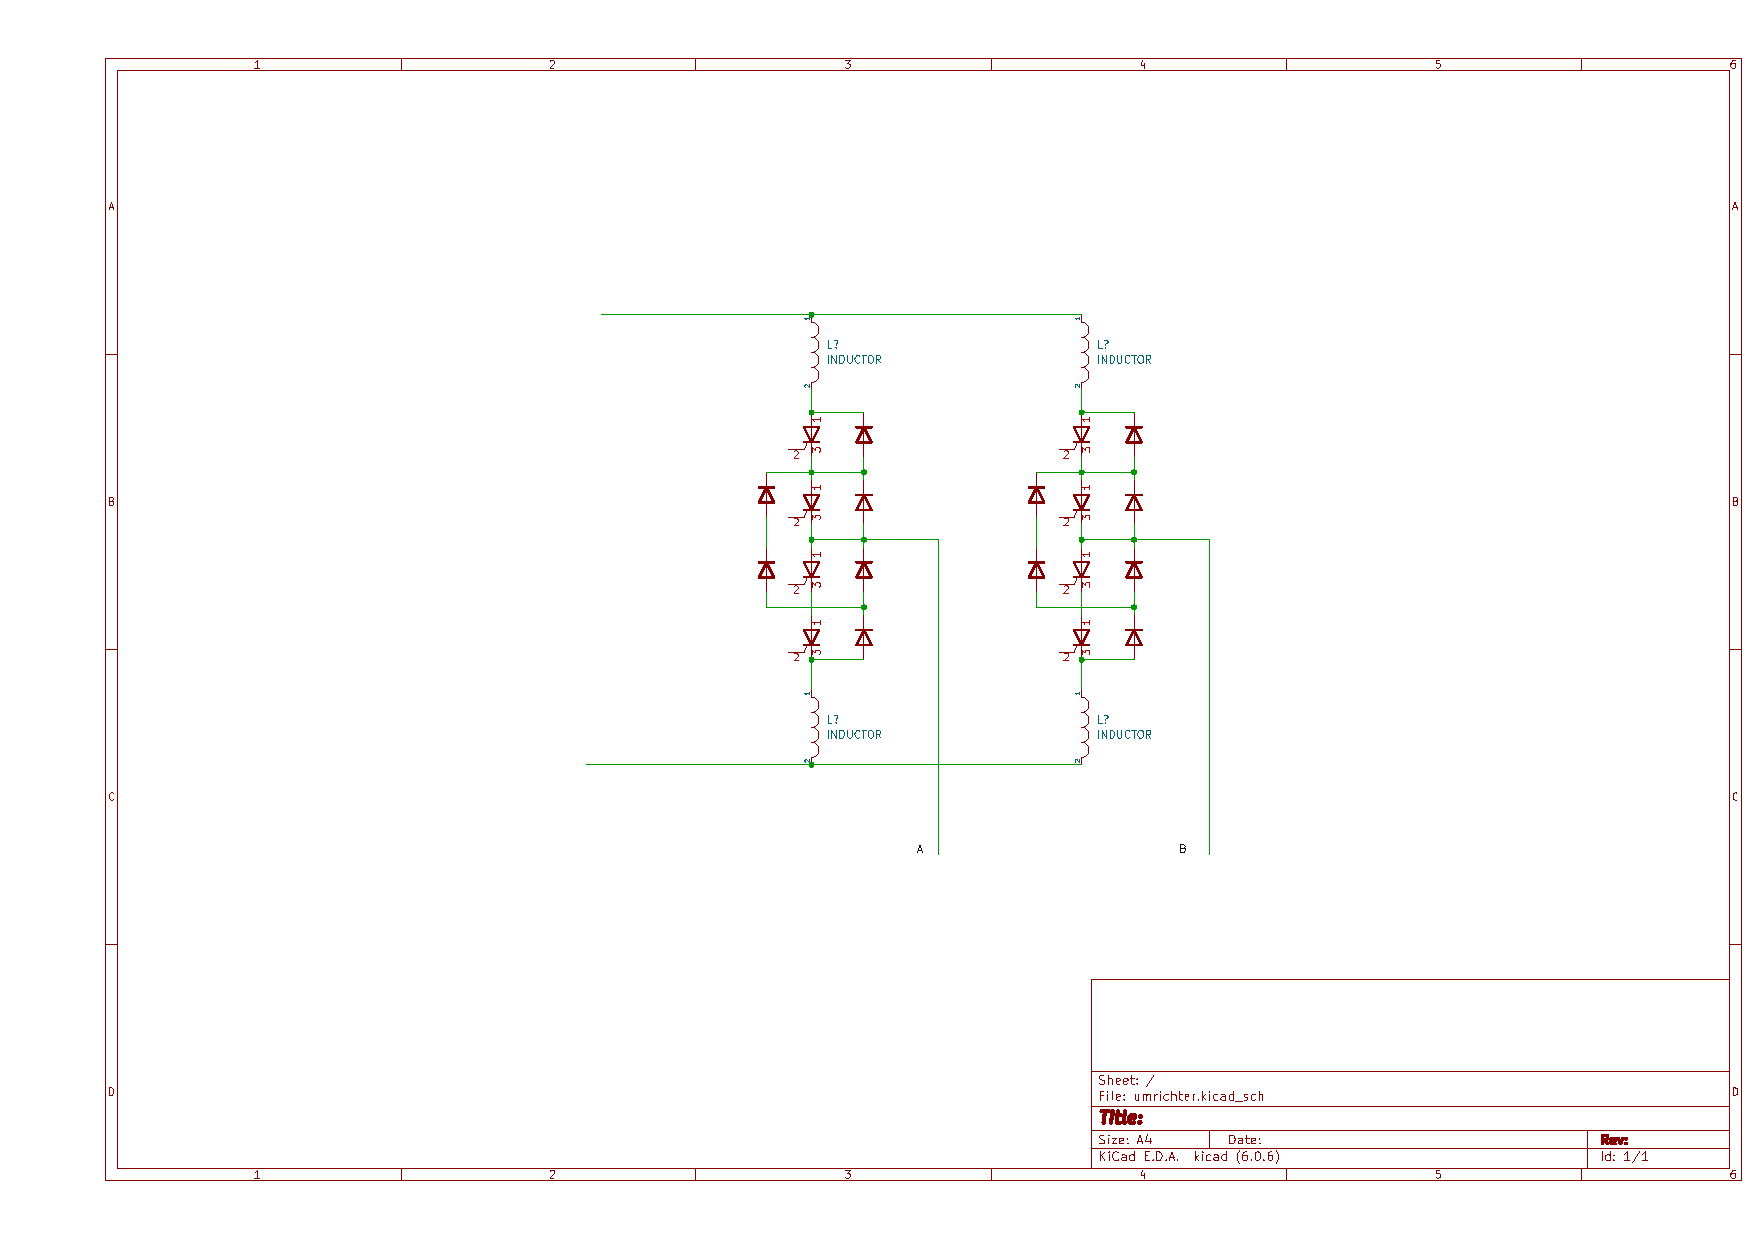
\includepdf[landscape]{Bilder/umrichter.pdf}
